\chapter{Counterfactuals supplementary}\label{chap:interpretability_appendix}

\begin{figure}[htbp]
	\centering
	\begin{subcaptiongroup}
		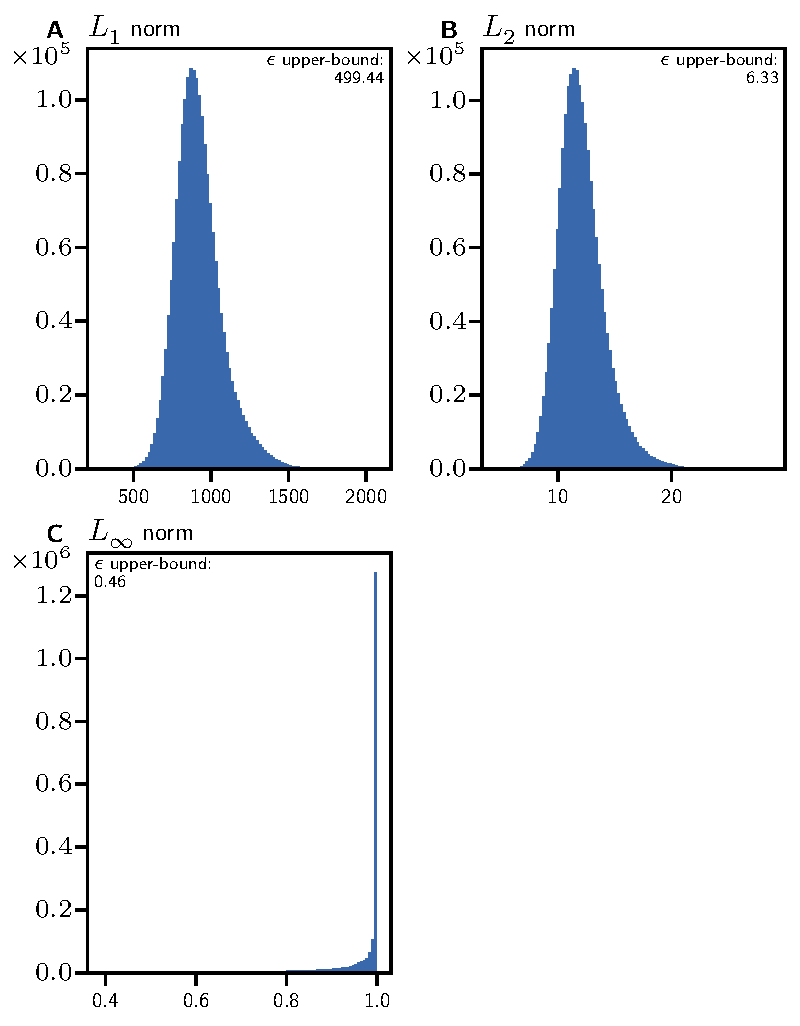
\includegraphics{distance_distribution_classes.pdf}
		\phantomcaption\label{fig:dist_cls_distibutionL1}
		\phantomcaption\label{fig:dist_cls_distibutionL2}
		\phantomcaption\label{fig:dist_cls_distibutionLinf}
	\end{subcaptiongroup}
	\caption{Distances distributions of points in two different classes}\label{fig:dist_cls_distibution}
\end{figure}

\begin{figure}[htbp]
	\centering
	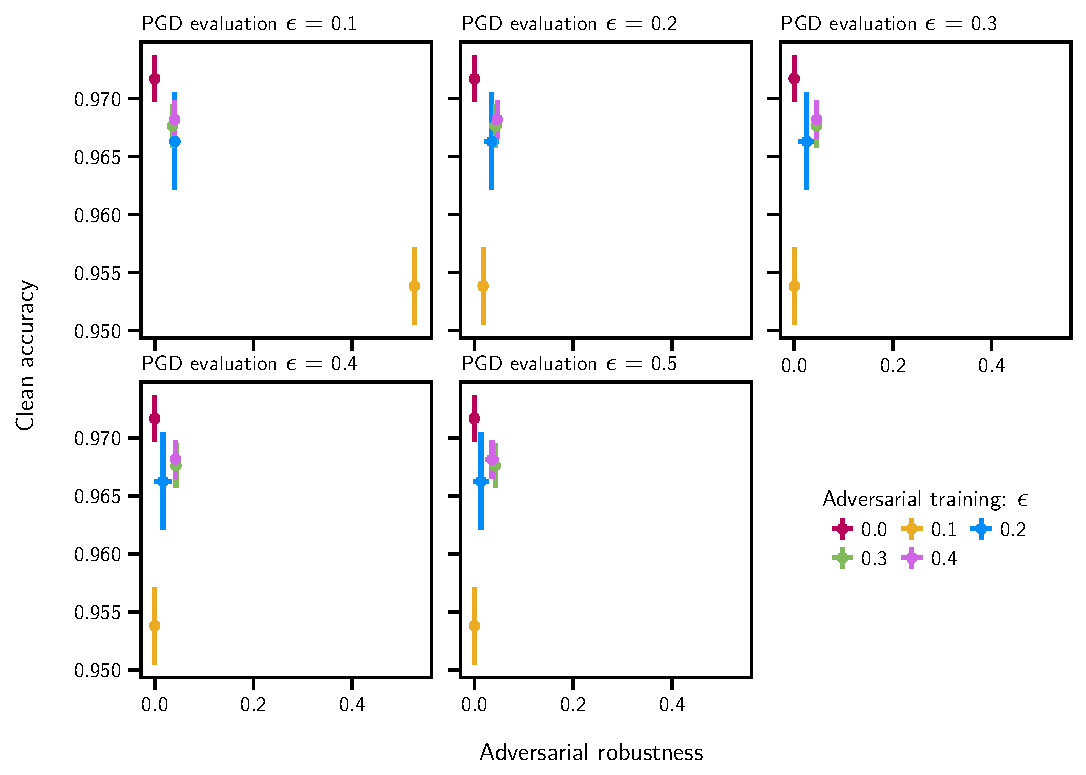
\includegraphics[scale=1]{MLP_LN_adversarial_tradeoff.pdf}
	\caption[\glsfmtshort{mlp} LN adversarial robustness-accuracy tradeoff]{Comparison of the adversarial robustness-accuracy tradeoff for \glsfmtshort{pgd} attacks with different sizes (\(\epsilon > 0\)) after adversarial training of the \glsfmtshort{mlp} LN model with various \glsfmtshort{pgd} attacks sizes, \(\epsilon = 0\) corresponds to a classical training on only clean samples. }\label{fig:mlp_ln_adv_tradeoff}
\end{figure}

\begin{figure}[htbp]
	\centering
	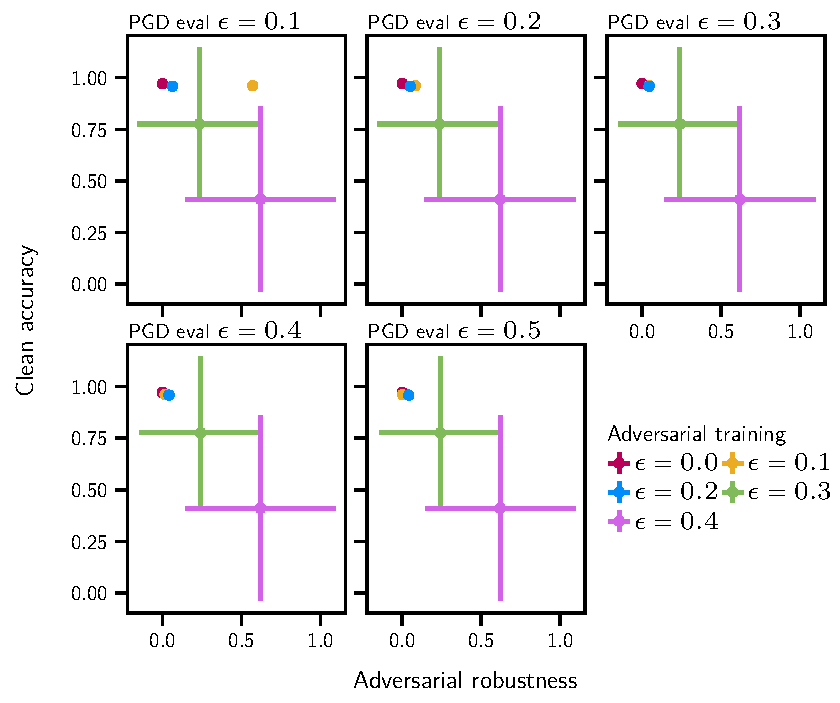
\includegraphics[scale=1]{MLP_NoNorm_adversarial_tradeoff.pdf}
	\caption[\glsfmtshort{mlp} NoNorm adversarial robustness-accuracy tradeoff]{Comparison of the adversarial robustness-accuracy tradeoff for \glsfmtshort{pgd} attacks with different sizes (\(\epsilon > 0\)) after adversarial training of the \glsfmtshort{mlp} NoNorm model with various \glsfmtshort{pgd} attacks sizes, \(\epsilon = 0\) corresponds to a classical training on only clean samples. }\label{fig:mlp_nonorm_adv_tradeoff}
\end{figure}

\begin{figure}[htbp]
	\centering
	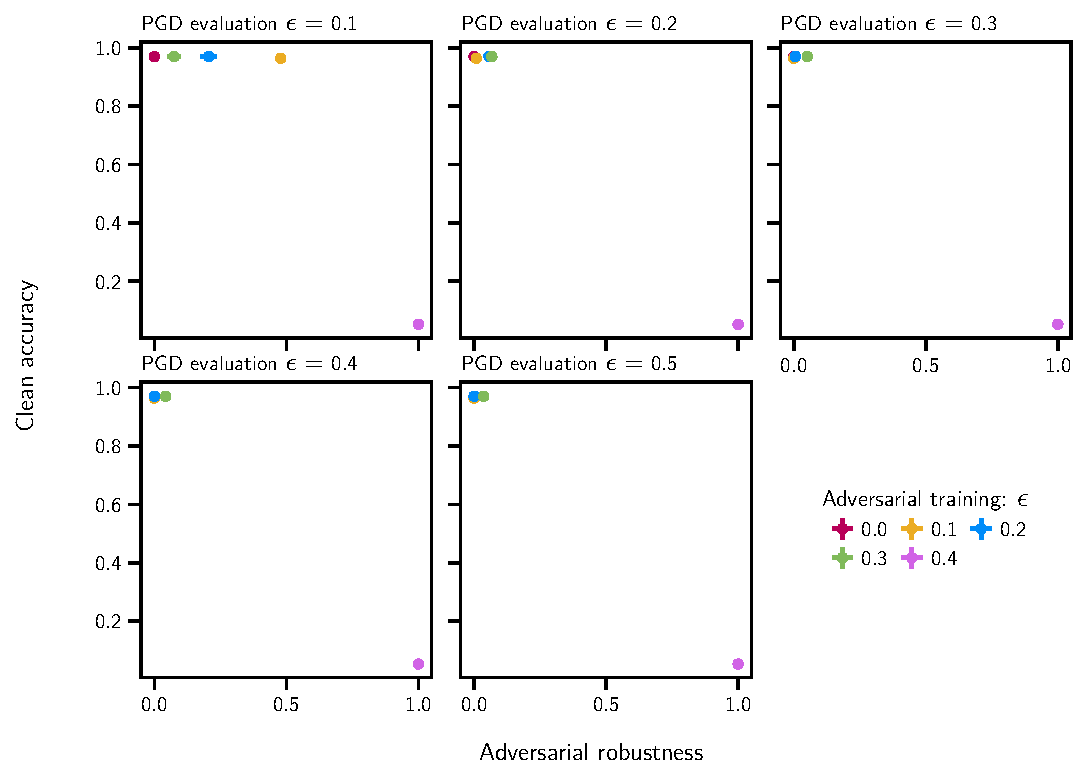
\includegraphics[scale=1]{MLP_FN_adversarial_tradeoff.pdf}
	\caption[\glsfmtshort{mlp} NF adversarial robustness-accuracy tradeoff]{Comparison of the adversarial robustness-accuracy tradeoff for \glsfmtshort{pgd} attacks with different sizes (\(\epsilon > 0\)) after adversarial training of the \glsfmtshort{mlp} NF model with various \glsfmtshort{pgd} attacks sizes, \(\epsilon = 0\) corresponds to a classical training on only clean samples. }\label{fig:mlp_fn_adv_tradeoff}
\end{figure}

\begin{figure}[htbp]
	\centering
	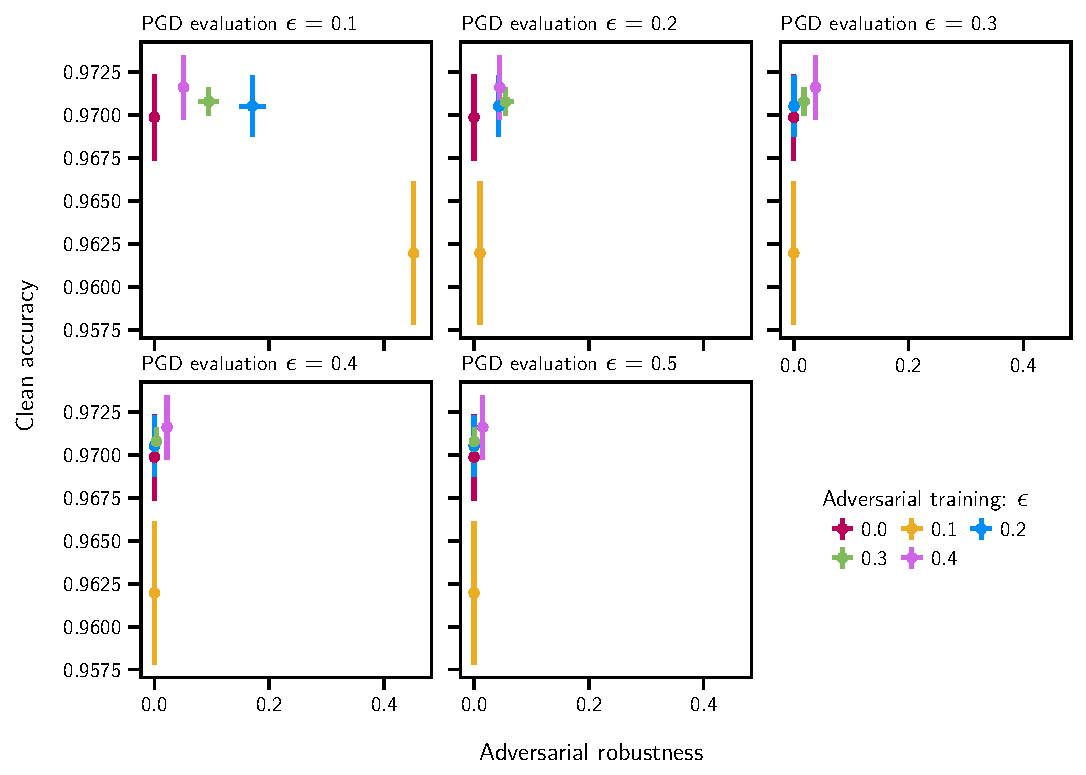
\includegraphics[scale=1]{MLP_FN_AGC_adversarial_tradeoff.pdf}
	\caption[\glsfmtshort{mlp} NF AGC adversarial robustness-accuracy tradeoff]{Comparison of the adversarial robustness-accuracy tradeoff for \glsfmtshort{pgd} attacks with different sizes (\(\epsilon > 0\)) after adversarial training of the \glsfmtshort{mlp} NF AGC model with various \glsfmtshort{pgd} attacks sizes, \(\epsilon = 0\) corresponds to a classical training on only clean samples. }\label{fig:mlp_fnagcadv_tradeoff}
\end{figure}


\begin{figure}[htbp]
	\centering
	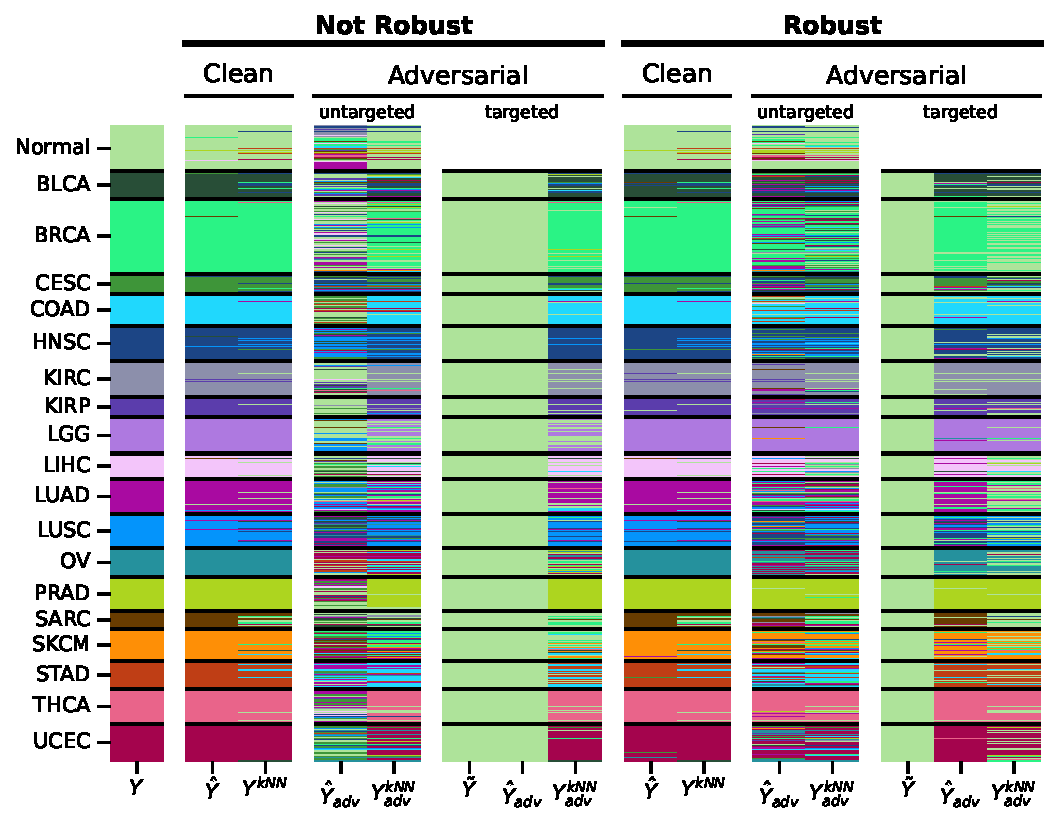
\includegraphics[width=\textwidth]{MLP_LN_knn_comparison.pdf}
	\caption[\glsfmtshort{knn} characterization of adversarial examples with \glsfmtshort{mlp} LN]{\glsfmtshort{knn} characterization of adversarial examples with \glsfmtshort{mlp} LN after clean training (Not Robust) and adversarial training (Robust). For both training strategies we compared untargeted and targeted attacks. \(Y\) represents the true label, \(\hat{Y}\) the predicted class by the model, \(Y^{\text{kNN}}\) the majority voting from the 20 nearest neighbors, \(\hat{Y}_{adv}\) the predicted class of the found adversarial example, \(Y^{\text{kNN}}_{adv}\) the majority voting from the 20 nearest neighbors of the found adversarial, and \(\tilde{Y}\) the desired class of targeted attackes. We set \(\tilde{Y}\) to normal for all samples.}\label{fig:mlp_ln_knn_comp}
\end{figure}

\begin{figure}[htbp]
	\centering
	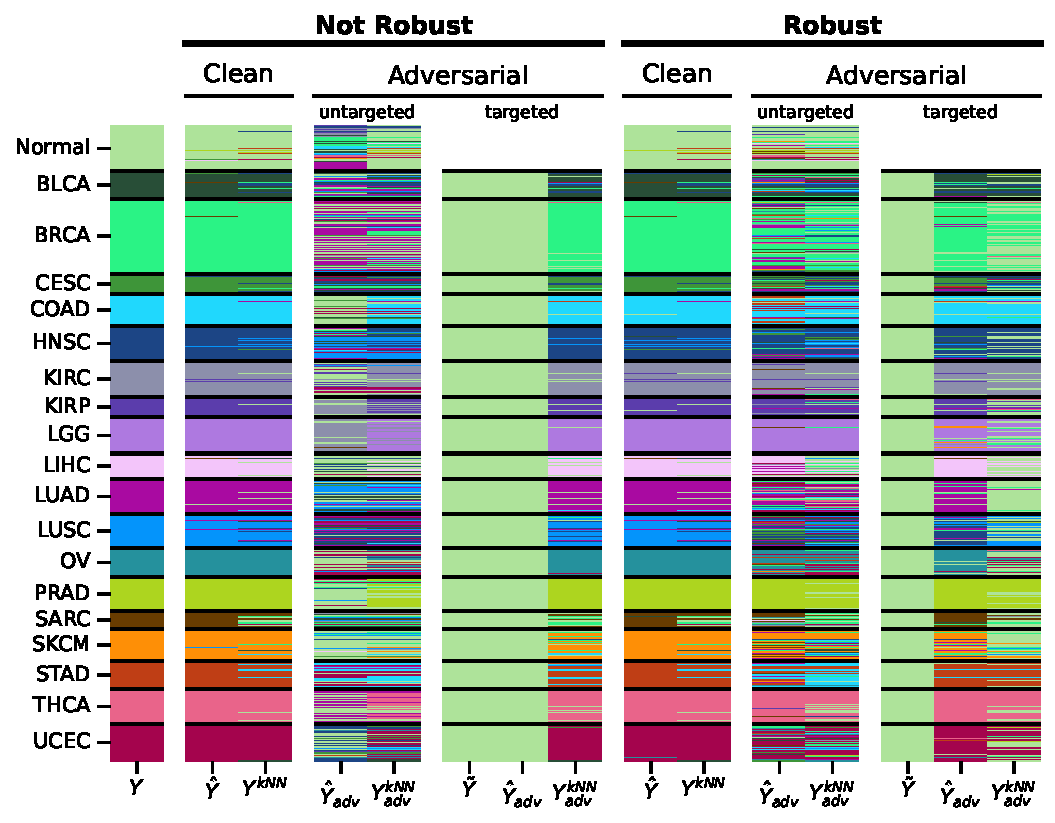
\includegraphics[width=\textwidth]{MLP_NoNorm_knn_comparison.pdf}
	\caption[\glsfmtshort{knn} characterization of adversarial examples with \glsfmtshort{mlp} NoNorm]{\glsfmtshort{knn} characterization of adversarial examples with \glsfmtshort{mlp} NoNorm after clean training (Not Robust) and adversarial training (Robust). For both training strategies we compared untargeted and targeted attacks. \(Y\) represents the true label, \(\hat{Y}\) the predicted class by the model, \(Y^{\text{kNN}}\) the majority voting from the 20 nearest neighbors, \(\hat{Y}_{adv}\) the predicted class of the found adversarial example, \(Y^{\text{kNN}}_{adv}\) the majority voting from the 20 nearest neighbors of the found adversarial, and \(\tilde{Y}\) the desired class of targeted attackes. We set \(\tilde{Y}\) to normal for all samples.}\label{fig:mlp_nonorm_knn_comp}
\end{figure}

\begin{figure}[htbp]
	\centering
	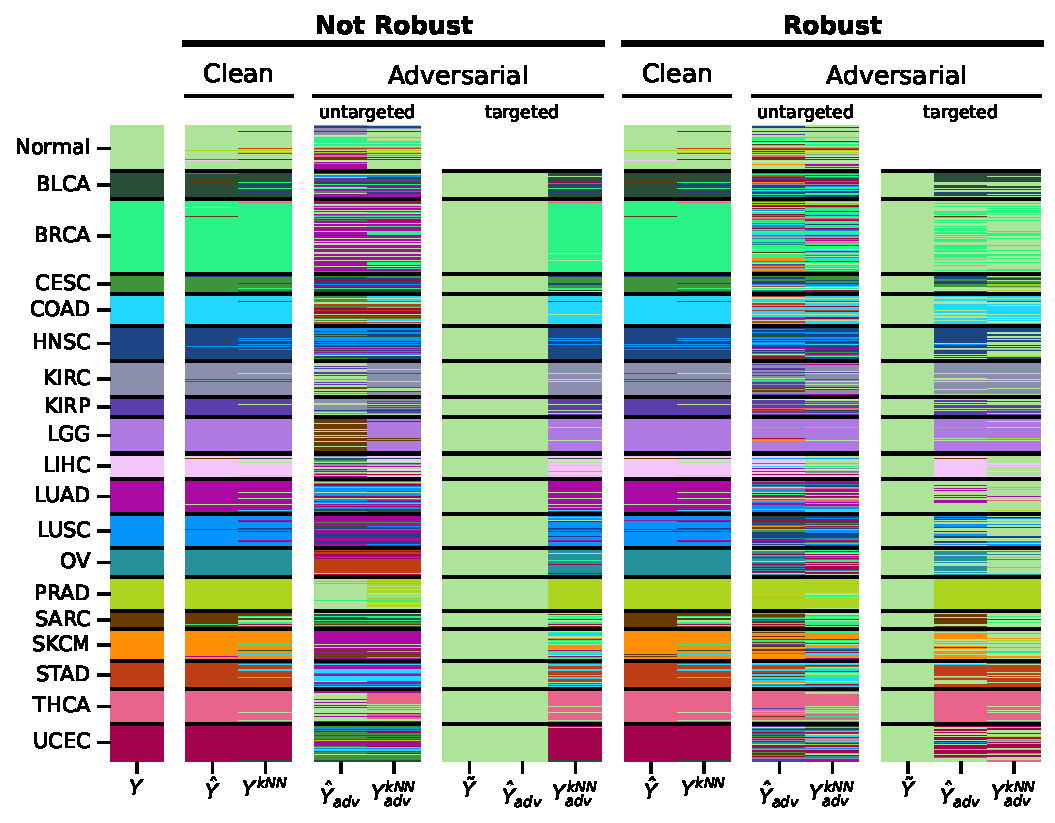
\includegraphics[width=\textwidth]{MLP_FN_knn_comparison.pdf}
	\caption[\glsfmtshort{knn} characterization of adversarial examples with \glsfmtshort{mlp} NF]{\glsfmtshort{knn} characterization of adversarial examples with \glsfmtshort{mlp} NF after clean training (Not Robust) and adversarial training (Robust). For both training strategies we compared untargeted and targeted attacks. \(Y\) represents the true label, \(\hat{Y}\) the predicted class by the model, \(Y^{\text{kNN}}\) the majority voting from the 20 nearest neighbors, \(\hat{Y}_{adv}\) the predicted class of the found adversarial example, \(Y^{\text{kNN}}_{adv}\) the majority voting from the 20 nearest neighbors of the found adversarial, and \(\tilde{Y}\) the desired class of targeted attackes. We set \(\tilde{Y}\) to normal for all samples.}\label{fig:mlp_fn_knn_comp}
\end{figure}

\begin{figure}[htbp]
	\centering
	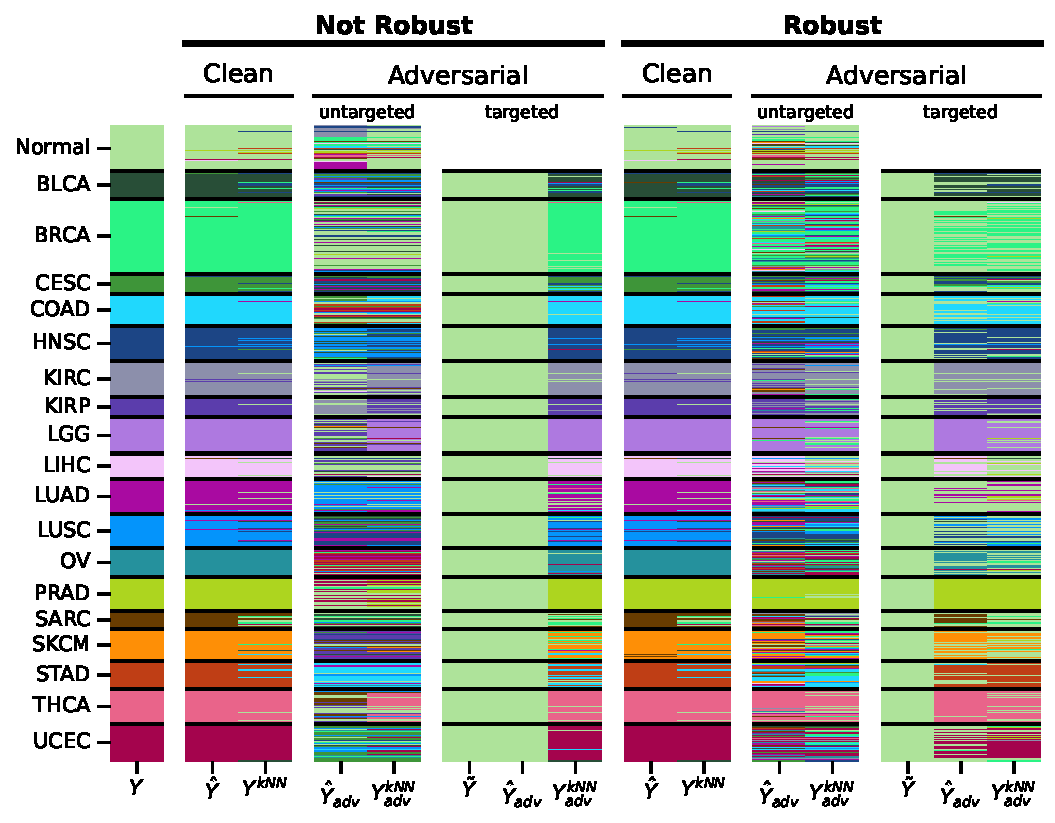
\includegraphics[width=\textwidth]{MLP_FN_AGC_knn_comparison.pdf}
	\caption[\glsfmtshort{knn} characterization of adversarial examples with \glsfmtshort{mlp} NF AGC]{\glsfmtshort{knn} characterization of adversarial examples with \glsfmtshort{mlp} NF AGC after clean training (Not Robust) and adversarial training (Robust). For both training strategies we compared untargeted and targeted attacks. \(Y\) represents the true label, \(\hat{Y}\) the predicted class by the model, \(Y^{\text{kNN}}\) the majority voting from the 20 nearest neighbors, \(\hat{Y}_{adv}\) the predicted class of the found adversarial example, \(Y^{\text{kNN}}_{adv}\) the majority voting from the 20 nearest neighbors of the found adversarial, and \(\tilde{Y}\) the desired class of targeted attackes. We set \(\tilde{Y}\) to normal for all samples.}\label{fig:mlp_fnagc_knn_comp}
\end{figure}